% --------------------------------------------------------------
% This is all preamble stuff that you don't have to worry about.
% Head down to where it says "Start here"
% --------------------------------------------------------------
 
\documentclass[11pt]{article}
 
\usepackage[margin=0.5in]{geometry} 
\usepackage{amsmath,amsthm,amssymb, enumerate, soul, float, multirow, varwidth, bm, hyperref}
\usepackage[hashEnumerators,smartEllipses]{markdown}
\usepackage{graphicx}
\usepackage[ruled,vlined]{algorithm2e}
\graphicspath{ {./images/} }
 
\begin{document}

% --------------------------------------------------------------
%                         Start here
% --------------------------------------------------------------
 
\title{Repository Analysis Report for Netron}
\author{Pengnan Fan \\ pengnan.fan@mail.mcgill.ca}

\maketitle

\section{Introduction}
In this report, I investigated an open source project (\href{https://github.com/openstack/neutron}{openstack/netron}) from GitHub and studied module-level file changes of its master branch in the past six month. For the study, the top-12 active modules are investigated by following standard: 1) number of commits and 2) number of edition (lines of add and delete). For this report, commit records are collected through GitHub API and visualized by a python script.

\section{Result}
According to my script, there are \textbf{490 commits} occurred in the past six month. These commits include at least one file change under the \textit{/neutron} directory of the studied project. According to table~\ref{tab:2}, the top-12 active modules \textbf{by number of commits} are test, db, plugins, agents, services, extensions, objects, cmd, quota, common, conf and api.
\begin{table}[H]
    \centering
    \begin{tabular}{|c||c|}
         \hline
         module & commit \\
         \hline
         tests & 773 \\
         db & 282 \\
         plugins & 267 \\
         services & 154 \\
         agent & 150 \\
         objects & 92 \\
         common & 54 \\
         conf & 40 \\
         extensions & 39 \\
         api & 33 \\
         cmd & 19 \\
         quota & 11\\
         \hline
    \end{tabular}
    \caption{Details for Top-12 Most Active Modules under /neutron by commits}
    \label{tab:2}
\end{table}
Interestingly, although the modules are the same, the rank is different when sorting them based on number of editions. According to table~\ref{tab:1}, the top-12 active modules \textbf{by number of editions} are test, plugins, db, agents, services, extensions, objects, cmd, quota, common, conf and api.
\begin{table}[H]
    \centering
    \begin{tabular}{|c||c|c|c|}
         \hline
         module & total edition & addition & deletion\\
         \hline
         test & 26556 & 19238 & 7318\\
         plugins & 6559 & 4275 & 2284\\
         db & 6303 & 4556 & 1747\\
         agent & 3827 & 2944 & 883\\
         services & 2786 & 1808 & 978\\
         objects & 1131 & 838 & 293\\
         extensions & 989 & 937 & 52\\
         cmd & 933 & 929 & 4\\
         quota & 560 & 178 & 382\\
         api & 523 & 314 & 209\\
         conf & 501 & 414 & 87\\
         common & 486 & 338 & 148\\
         \hline
    \end{tabular}
    \caption{Details for Top-12 Most Active Modules under /neutron by edition}
    \label{tab:1}
\end{table}
In addition, I also visualized the top-12 active modules by editions and commits. Due to space limit, you may find more visualizations from the jupyter notebook.
\begin{figure}[H]
    \centering
    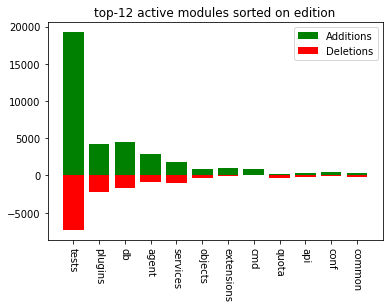
\includegraphics[width=0.5\linewidth]{./img/sorted_by_edition/top-12_active_modules_sorted_on_edition_bar.png}
    \caption{Bar Chart for Top-12 Active Modified Modules under /neutron by editions}
    \label{fig:1}
\end{figure}
\begin{figure}[H]
    \centering
    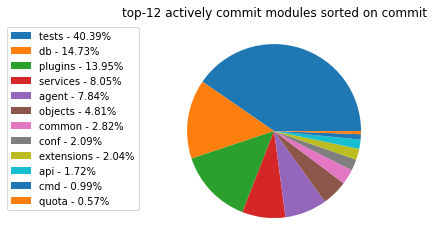
\includegraphics[width=0.5\linewidth]{./img/sorted_by_commit/top-12_actively_commit_modules_sorted_on_commit_pie.png}
    \caption{Pie Chart for Top-12 Active Modified Modules under /neutron by commits}
    \label{fig:2}
\end{figure}


\end{document}